
\documentclass[a4paper,12pt]{article}
\usepackage{fullpage}
\usepackage{multirow}
\usepackage{graphicx}
\usepackage{float}
\usepackage{color}
\usepackage{caption}
\usepackage{tabularx}
\usepackage{subcaption}
%\usepackage{subfigure}
\usepackage{subcaption}
%\restylefloat{table}
%\floatstyle{boxed}
\captionsetup{font={footnotesize}, labelfont={footnotesize}}


\begin{document}

Daniel Reid, BBM iteration assignment

\section{Background} 
	\paragraph*{}
		The purpose of this assignment is to compare the leapfrog and predictor-corrector schemes in modeling a low amplitude wave using the Benjamin-Bona-Mahony (BBM) partial differential equation, and to describe the model's accuracy and computation time with respect to time and position step size.  The BBM equation is shown in equation \ref{eq:BBMDiff}.
			\begin{equation}
				\label{eq:BBMDiff}
				u_{t} + u{x} + uu_{x} - u_{xxt} = 0
			\end{equation}
		The time derivative can be isolated as shown in Equation \ref{eq:BBMSolvedUt}.
			\begin{equation}
				\label{eq:BBMSolvedUt}
				u_{t}=-(1-\frac{d^{2}}{dx^{2}})^{-1}\frac{d}{dx}(u+u^{2}) = B(u+u^{2})
			\end{equation}
		Equation \ref{eq:BBMSolvedUt} can be iterated using matrices to describe $\frac{d}{dx}(u+u^2)$ and $(1-\frac{d^{2}}{dx^{2}})^{-1}$.  
		\paragraph*{} A center differencing scheme is used to take the derivative of $u+u^{2}$.  The matrix populates $\frac{1}{2dx}$ on the upper diagonal and $\frac{-1}{2dx}$ on the lower diagonal.  

			  The result of the matrix operating on $u+u^{2}$ is shown in Equation \ref{eq:derivative}.
			\begin{equation}
				\label{eq:derivative}
				\frac{d(u+u^{2})_{i}}{dx} = \frac{(u+u^{2})_{i+1} - (u+u^{2})_{i-1}}{2dx}
			\end{equation}

		The matrix describing $1-\frac{d^{2}}{dx^{2}}$ populates the upper and lower diagonals with $\frac{-1}{dx^{2}}$, and the main diagonal with $1 + \frac{2}{dx^{2}}$.
	\paragraph*{}
		The iterating loop for the predictor corrector methods is shown below,
		\begin{verbatim}
			def iteratePredCor(nts, yuMtx, dt, invSvm, fod):
				   for t in range(nts):
			       prediction = yuMtx + eulerStep(dt, invSvm, fod, yuMtx)
				      	yuMtx = .5 * (prediction + yuMtx + eulerStep(dt, invSvm, fod, prediction))
			return yuMtx
		\end{verbatim}
	\paragraph*{}
		where eulerStep is defined as 
		\begin{verbatim}
		def eulerStep(dt, invSvm, fod, yuMtx):
	   		return -dt * (invSvm * (fod * (yuMtx + sqrVals(yuMtx))))

		\end{verbatim}
	\paragraph*{}
		The iterating loop for the leapfrog method is shown below.
		\begin{verbatim}
		def iterateLeapFrog(nts, yuMtx, dt, invSvm, fod):
		   	yuLast = yuMtx.copy()
		   	yuMtx = iteratePredCor(1, yuMtx, dt, invSvm, fod)
		   	nts-=1
		   	for t in range(nts):
		      		store = yuMtx.copy()
			      	yuMtx = yuLast + 2 * eulerStep(dt, invSvm, fod, yuMtx)
			      	yuLast = store
			return yuMtx
		\end{verbatim}
	\paragraph*{}
		The leapfrog method must store a copy of the last step, so two copies of the height list must be maintained. 
	\paragraph*{} 
		The BBM equation can be integrated into equation \ref{eq:BBMSolved}
		\begin{equation}
			\label{eq:BBMSolved}
			u(x, t) = \frac{3}{2}asech^{2}(\frac{1}{2}\sqrt{\frac{a}{a+1}}(x-(1+a)t))
		\end{equation}
		where $a$ is the amplitude of the wave.  This is used to evaluate the results of the iterations.

\section{Results}
	\paragraph*{}
		The results are shown in the table below.
		\begin{center}\label{table:Results}
			\begin{tabular}{l | c | c | c | c | c}
				 & Relative max error & dx & dt & nts & seconds\\
				 \hline
				 Pred/cor & \begin{tabular}{c}1.93E-3\\6.40E-5\\3.40E-4\end{tabular} &
				  \begin{tabular}{c}0.2\\0.1\\0.05\end{tabular} & 
				  \begin{tabular}{c} 0.04\\0.04\\0.04\end{tabular} & 
				  \begin{tabular}{c} 600\\600\\600\end{tabular}  &
				  \begin{tabular}{c} 9\\19\\41\end{tabular} \\
				  \hline
				Pred/cor & 
				\begin{tabular}{c}6.40E-5\\4.70E-4\\5.60E-4\end{tabular} &
				  \begin{tabular}{c}0.1\\0.1\\0.1\end{tabular} & 
				  \begin{tabular}{c} 0.04\\0.02\\0.01\end{tabular} & 
				  \begin{tabular}{c} 600\\1200\\2400\end{tabular}  &
				  \begin{tabular}{c} 19\\38\\76\end{tabular} \\
				  \hline
				 Leapfrog & \begin{tabular}{c}2.01-3\\8.60-5\\3.36-4\end{tabular} &
				  \begin{tabular}{c}0.2\\0.1\\0.05\end{tabular} & 
				  \begin{tabular}{c} 0.04\\0.04\\0.04\end{tabular} & 
				  \begin{tabular}{c} 600\\600\\600\end{tabular}  &
				  \begin{tabular}{c} 5\\9\\21\end{tabular} \\
				  \hline
				Leapfrog & 
				\begin{tabular}{c}8.60E-5\\4.61E-4\\5.56E-4\end{tabular} &
				  \begin{tabular}{c}0.1\\0.1\\0.1\end{tabular} & 
				  \begin{tabular}{c} 0.04\\0.02\\0.01\end{tabular} & 
				  \begin{tabular}{c} 600\\1200\\2400\end{tabular}  &
				  \begin{tabular}{c} 9\\19\\38\end{tabular} \\
				  \hline
			\end{tabular}
		\end{center}
		The results show that computation time scales linearly with number of time steps, which is expected since increasing the number of time steps does not increase the complexity of each time step.  Computation time also scales roughly linearly with position step size, which is unexpected because the time to solve the next step should scale roughly with the number of elements in svm matrix, $\propto \frac{1}{dx^{2}}$.  The lowest error was not at the smallest length step size.  A small step size would give a large difference in the order or magnitude between the values in the $fod$ and $svm^{-1}$ matrices, which could introduce numerical error.  The leapfrog method runs roughly twice as quickly as the predictor-corrector method, since a predictor-corrector is roughly twice as complex.  The accuracy of the leapfrog method is roughly the same as that of the predictor-corrector method.  It is possible they would diverge more in longer simulations, but inverting matrices for longer waves took too long.  The relative max error was calculated using Equation \ref{eq:err},
		\begin{equation}
			\label{eq:err}
			maxErr = \frac{abs(a[i] - b[i])}{avg(a[i], b[i])}
		\end{equation}
		where a is the exact height list, b is the iterated height list, and i is the index of a's maximum.
	\paragraph*{}
		The run times in this simulation are much slower than those in the class example implemented in Octave.  This is probably Octave uses native code for its matrix operations while the libraries used here are implemented in Python.  These Python libraries are likely slower since they are interpreted rather than compiled.  
	\paragraph*{}
		Some sample graphs are shown below.
	\begin{center}
		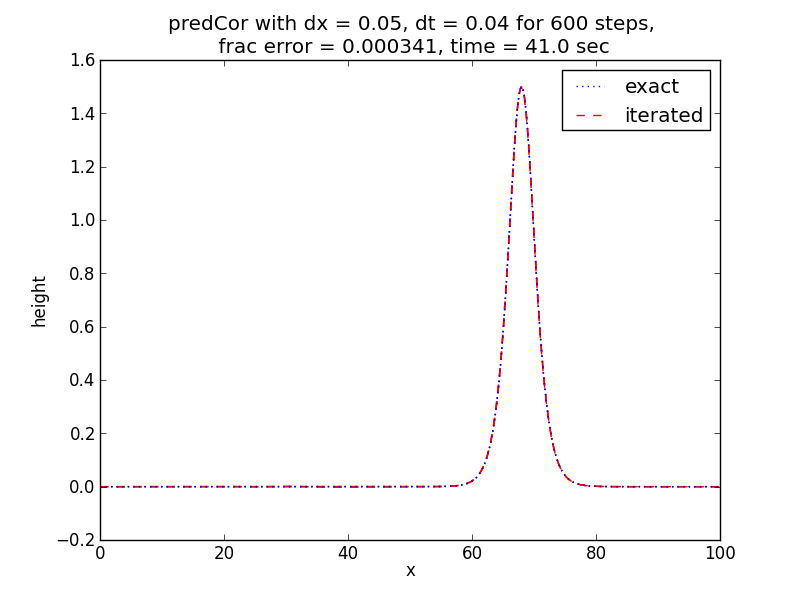
\includegraphics[width=11cm]{output2}
		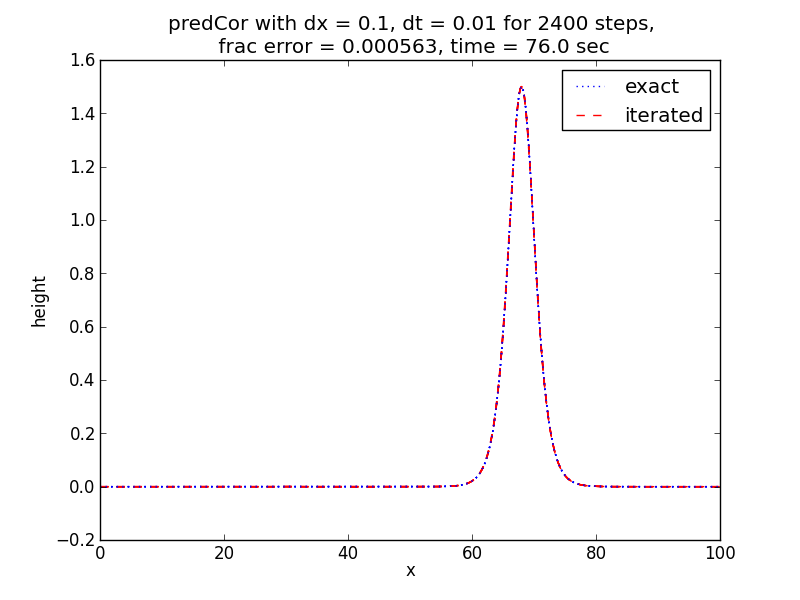
\includegraphics[width=11cm]{output5}
		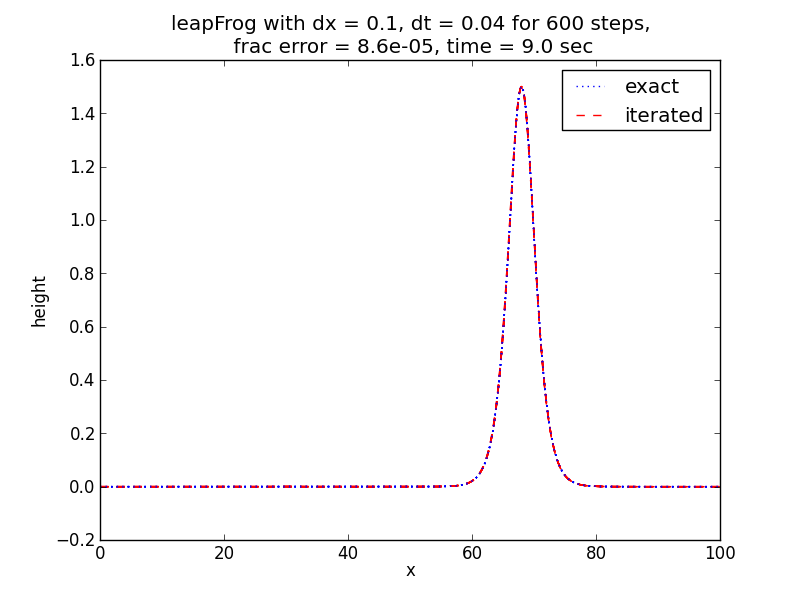
\includegraphics[width=11cm]{output9}
	\end{center}



\end{document}